\documentclass[11pt]{article}
\usepackage{geometry}
\geometry{a4paper} 
\usepackage{amssymb}
\usepackage[pdftex]{graphicx}
\usepackage{color}
\definecolor{dkgreen}{rgb}{0,0.6,0}
\definecolor{gray}{rgb}{0.5,0.5,0.5}
\definecolor{mauve}{rgb}{0.58,0,0.82}
\definecolor{paleblue}{rgb}{0.2,0.5,0.82}
\usepackage{listings}
\lstset{language=C, breaklines=true, basicstyle=\footnotesize\ttfamily, tabsize=4}
\usepackage[font=small, font+=it]{caption}
\usepackage{url}
\usepackage{mdwlist}
\usepackage{subfigure}
\usepackage{mdwmath}
\usepackage{amsmath}


\title{Audio Programming 4\\Audio Visualiser}
\author{0800706M}
\date{\today}

\begin{document}
\maketitle
\begin{abstract}
This paper presents a novel method of visualising digital audio signals. It is intended be aesthetically engaging, and also display a faithful representation of the original audio. The images created offer a sense of the spectral and temporal properties of the audio, with a general emphasis being artistic rather than analytic. Additionally, basic keyboard interaction is introduced to allow the user to tailor the visual output based on the particular audio input and personal taste.
\end{abstract}

\section{Concept}
The basis of the visualiser is the Hilbert transform. This is a linear operator which, when applied to a given real function $f(t)$, returns a function $\hat{f}(t)$ which has a $\frac{\pi}{2}$ radian phase-shift and is orthogonal to the original function. Mathematically it is defined as:
\begin{equation}
	\hat{f}(t) = \frac{1}{\pi}P\int_{-\infty}^{\infty}\frac{f(\tau)}{t-\tau}d\tau \quad \textrm{if the integral exists}
\end{equation}
where $P$ is the Cauchy principal value. The mathematical proof and implementation are beyond the scope of this report, but are discussed in detail by Mathias Johansson (1999)\cite{mj}. The Python scipy library provides a function to calculate the Hilbert transform of a number array, which returns a set of complex numbers with the real parts representing the original signal, and the imaginary parts representing the Hilbert transform.

The Hilbert transform is more commonly used to transform a real signal into a so-called ``strong analytic signal''. Using the fact that $f(t)$ and $\hat{f}(t)$ are orthogonal, standard complex number arithmetic can be used to give the instantaneous amplitude and phase. This in turn can be thought of as the sum of many rotating vectors, each representing a single frequency component. Hence, plotting this instantaneous vector on an argand diagram as it rotates in time generates interesting visual patterns that directly represent the original audio signal.
\newpage The following basic steps are the algorithm for generating each frame of video:
\begin{enumerate*}
	\item Get audio buffer from sound card.
	\item Calculate colour to display based on RMS level of audio.
	\item Perform Hilbert transform on audio vector.
	\item Scale and shift to fit onto window.
	\item Filter to remove sharp corners and other artifacts.
	\item Convert to list of $(x,y)$ co-ordinates for plotting.
	\item Draw black rectangle with high transparency.
	\item Draw line joining all co-ordinates.
	\item Draw text if needed.
\end{enumerate*}

\section{Python Implementation}
In the following sections, numbers in square parentheses refer to lines of the code found in appendix \ref{app:code}. 

\subsection{The World}
In order to draw images in a window, the Pyglet library was used\cite{pyglet}. This is essentially a wrapper around the OpenGL drawing functions\cite{opengl}, and also includes ways to schedule updates, control the frame rate, and other useful functions.

The basis of the entire application is the Window class in the pyglet.window library. This class has several special functions that it understands, but still must be programmed before anything is displayed. Hence, Window is used as the base of the World class. This solves many problems associated with defining the special Window functions, as the World class inherits these functions and they can be defined within World. It also allows for effective time keeping, as the `dt' [108] value denoting the time since the last update can be accumulated as an attribute of the World, rather than using a global variable.

On initialisation of the World, the Window's \_\_init\_\_() function is called in order to generate the actual window [26]. Following this, the window is cleared, OpenGL and scheduler settings are given, the needed variables and objects are declared, and the audio stream is opened.


\subsection{Real--time audio}
Raw audio data is obtained using two separate modules. Firstly, the PyAudio python module is used to open an audio stream and return raw data\cite{pyaudio}. Secondly, the Soundflower application generates a virtual sound card that PyAudio can read from\cite{soundflower}. The sound output of the computer is also routed to Soundflower so that any sound heard on the speakers is also sent to the visualiser application.

A PyAudio stream is opened with minimal options [51--56], as most of the default settings are adequate for this application. The options used are: 16-bit integer sample values, 1 channel, 44.1kHz sample rate, input active, output inactive, and 1024 samples per audio frame. The audio vector size was chosen as a trade-off between fast reaction-time and preventing audio buffer overflow. Only one channel is used because a typical audio recording played into the visualser will not have particularly disparate stereo channels. For reasons discussed in section \ref{sec:filter} a better response is obtained from lower frequencies, which tend to be panned towards the centre. These factors, in conjunction with the high processing needs of the application, influenced the decision to ignore the other stereo channel. All other values are standard.

A function get\_audio() [80--90] is defined to retrieve audio samples from the stream. The data obtained from PyAudio is formatted by default as a single string with consecutive pairs of bytes representing a 16-bit audio sample. Hence the numpy.frombuffer() and numpy.array() functions are used to convert the string into individual sample values.

Due to the time between calls to get\_audio() not being strictly defined, (it depends on the render time of the video), some error handling must be introduced to ensure that the application does not throw an exception during buffer overruns. If an exception occurs, the error message is checked to see if it was due to an overrun, and either raised or passed depending on the result. If the exception was due to an overrun, it is assumed that all audio samples are zero.

\subsection{Audio processing}
As previously mentioned, the basis of the DSP chain is the scipy.signal.hilbert() function. In addition to this, several custom classes and functions were created to perform some basic tasks.
\subsubsection{Slide filter}
\label{sec:filter}
The slide filter smooths signal logarithmically between changes in sample values\cite{slide}. The equation is given by:
\begin{equation}
y[n] = y[n-1]+\frac{x[n]-y[n-1]}{a} \quad \textrm{for } a\ge1
\end{equation}
where $x$ is the input, $y$ is the output, and $a$ is the slide value.

It was decided to use this filter over one from a pre-existing library for several reasons. Firstly, a custom class retains sample values from the previous audio vector, which (assuming a buffer overrun does not occur), minimises the distance between the beginning of a line and the end of the previous one. Scipy functions generally created undesired transient effects at the beginning of the lines.

Secondly, this filter is extremely simple, and does not require the processing power associated with FFT filters or their equivalent time--domain convolution operations. Lastly, it looked better on--screen than a normal one--pole or biquad low--pass filter, and as it did not need to filter to any frequency specification, the `look' was deemed the most important factor.

The Silde\_filter class itself comprises of a 2-sample buffer to save the current and previous outputs. It has also been designed to perform the filter operation on an entire audio vector in order to keep processing styles constant throughout all sections of the DSP chain.

This filter had the added bonus of segregating frequencies in the image. That is to say that because higher frequencies are damped, they tend as generate curves in the centre of the image, and lower frequencies spread the curves toward the edges. While this is not a strict rule, and was not true in all cases, the general effect proved aesthetically pleasing.

\begin{figure}[htb]
\centering
\subfigure[Without filtering]{
	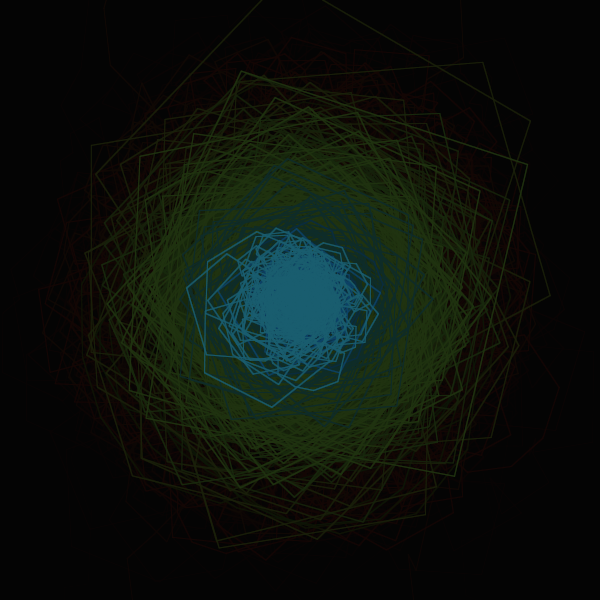
\includegraphics[width=0.3\textwidth]{images/no_filter.png}
	\label{fig:without}
}
\subfigure[Scipy filters]{
	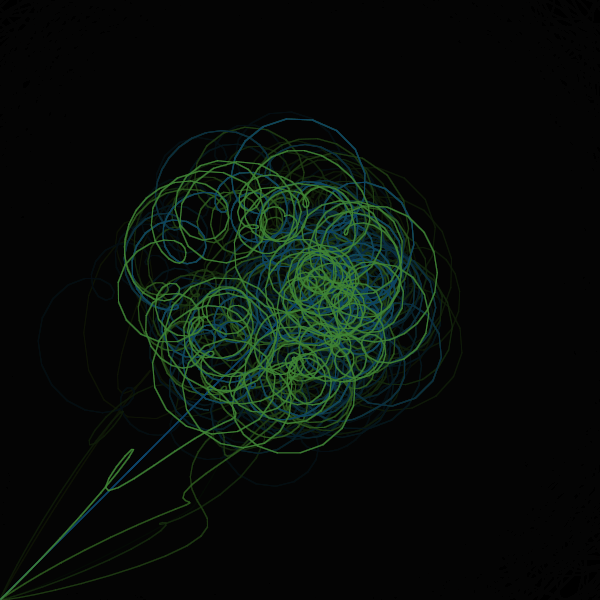
\includegraphics[width=0.3\textwidth]{images/iir.png}
	\label{fig:iir}
}
\subfigure[Slide filter]{
	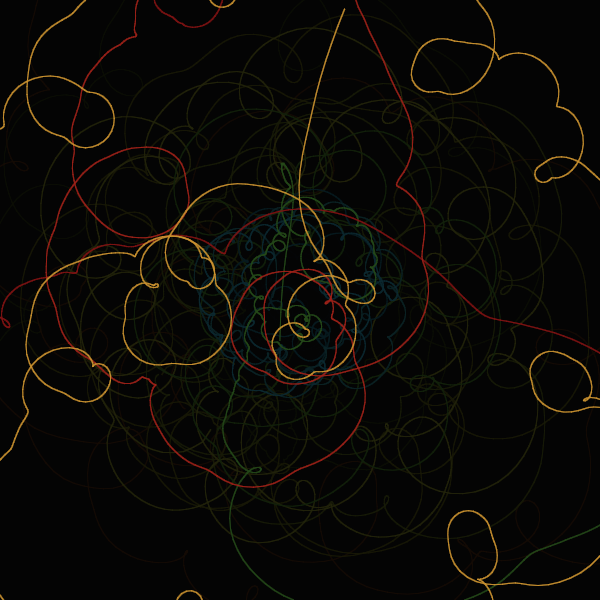
\includegraphics[width=0.3\textwidth]{images/slide.png}
	\label{fig:slide}
}
\label{fig:filtering}
\caption{Screenshots showing typical unsuccessful \subref{fig:without} \subref{fig:iir} and successful \subref{fig:slide} filtering.}
\end{figure}

\subsubsection{RMS}
\label{sec:rms}
In order to introduce colour to the visualiser, the average power value was used to select a display colour. A function, rms() [172--174], was introduced to calculate the root--mean--square value of the audio buffer. The RMS was calculated thusly:
\begin{equation}
x_{rms} = \sqrt*{\frac{1}{n}\sum_{i=0}^{n} (x_{i})^{2}}
\end{equation}
where $x$ is a single audio sample. In practice, the audio buffer was also heavily scaled in order to reduce the range of the RMS to something close to $0\le \textrm{RMS} \le 1$. The \emph{exact} boundary values were not important.

\subsection{Drawing}
All drawing is performed by OpenGL commands, and is scheduled by the Pyglet clock. This works efficiently by transferring relatively short lists of vertices to video RAM, and commanding OpenGL to interpret and draw them using the graphics processor, thereby freeing the CPU and allowing it to handle all the other tasks.

\subsubsection{Calculating vertices}
The hilbert() function returns a list of complex numbers, which are subsequently filtered. As Python stores complex numbers in $a+jb$ format, they can already be interpreted as co-ordinages on an argand diagram. Vertices should generally fall between 0 and the width/height of the Window (measured in pixels), so the buffer is scaled using the World's `self.scale' variable. It is also shifted by half the width and height of the window to bring the origin into the centre [99--101].

As an extra, the standard `oscilloscope style' waveform can be viewed. The vertices for this are calculated from the absolute value of the post-filter audio sample, and its index within the buffer. Again, they are scaled to fit the window, and shifted to the centre [102-106]. The buffer is also downsampled by half, as this number of data points fitted conveniently on the window.

In both of these cases, the filtered buffer is unpacked into a tuple of floats, with each subsequent pair representing an $x$ and $y$ co-ordinate.

\subsubsection{Drawing to the window}
As with many audio visualisers, it was desirable to emulate the persistence--of--vision effects of old CRT type monitors. To this end, at the start of each frame, a black polygon with an opacity of 10\% is drawn over the entire window [64--68]. Over many frames, this gives the impression that the audio trace is fading away.

Depending on the `self.mode' variable, one or both of the vertex lists and their associated colour tuples are passed to the pyglet.graphics.draw() function [69--75]. This has the effect of drawing a `GL primitive' to the window. There are several types of primitive, but in this case, a simple line joining all vertices is chosen. This is all that is required to display the audio waveform.

Text can also be displayed, depending on whether it is scheduled or not [76--78]. Since only one piece of text is to be displayed at one time, a variable `self.last\_text' is defined, which is compared to the current time. If the current time is less than one second after the last text update, the text is refreshed. If not, it is left to fade naturally. 

\subsection{Extra functionality}
\subsubsection{Colour interpolation}
As mentioned in section \ref{sec:rms}, the RMS value of the audio is used to determine the colour of the line being drawn. This value is then used as an interpolating index into an array of RGB colour values. The colours were chosen purely subjectively, and then arranged as a list of tuples, with the `quietest' one first [177--180].

Seeing as the there are four colours to interpolate between, each is given an equal sector of the range $0 \le \textrm{index} \le 1$. It is then assumed that the midpoint of a sector represents a pure colour with no interpolation. Given this, the interpolation index is calculated and the two colours to interpolate between are determined. The fractional part of the index is then used as a blend value, which determines how much of each colour to include in the final value: $c_{out} = c_2b+c_1(1-b)$ where $c$ is a colour, and $b$ is the blend value.

\emph{Note: Since the Hilbert transform gives the instantaneous amplitude, it was attempted to give each point a different colour. In practice however, this proved too slow to render, which resulted in constant buffer overruns. This method was therefore rejected.} 

\subsubsection{Keyboard input}
It is inevitable that different audio files will have different sonic properties. This is the motivation behind giving the user some form of control over the display. The on\_key\_press() function inherited from the Window class is used to implement this [111--134]. The user has control of the scaling of the visualiser, as well as the amount of filtering performed on the audio.

As a small extra, the keyboard input also offers options to hold the visualiser steady; switch between the hilbert display, waveform display, or both; and to save the current frame as PNG image. A message is displayed on the screen when any of the key actions are invoked.

\subsubsection{Screenshots}
A Screenshot\_saver class is defined in order to save a image [151--168]. The first task is to create a folder to hold the screenshots if one does not already exist. The Python os library has functions to do exactly this [154--156].

When the save\_image() function is invoked, the current video buffer is obtained from the Pyglet Buffer\_manager class. As OpenGL has been setup to use alpha blending, the alpha channel must be stripped from the screenshot, otherwise all black areas appear as transparent in the PNG image. This is done simply by setting the `format' attribute of the Image\_data object.

The Python datetime library is then used to construct a filename that contains the exact time and date. This prevents overwriting any current screenshots. Finally, the function returns a string depicting whether the file has been saved successfully or not. As with the get\_audio() function, the exceptions must be handled correctly to prevent the application crashing if the file is not saved for any reason.

\newpage
\section{Conclusion}
The application presents an alternative method of visualising pure audio data. The patterns vary greatly depending on the audio input used, such that while the visualiser is predictable, it remains appealing over prolonged use. The ability of the user to alter the behavior slightly in real-time, and save screenshots adds interactivity for the user.
\\ \\ Some improvements can be made with further development:
\begin{itemize*}
\item The audio could be upsampled to give more co-ordinates, and hence smoother lines at higher frequencies. This could require `thinning' of the vertex list to remove unnecessary co-ordinates.
\item The application could play an audio file as opposed to simply taking input from a sound card.
\item The parameters of the animation could vary over time, allowing an even more interesting visual experience. 
\end{itemize*}
\vspace{2cm}
\bibliographystyle{ieeetr}
\bibliography{audio_visualiser}

\newpage


\begin{appendix}
\section{Example screenshots}
\begin{figure}[h]
\centering
\subfigure[James Blake -- Limit to Your Love: Sub bass and minimal drums]{
	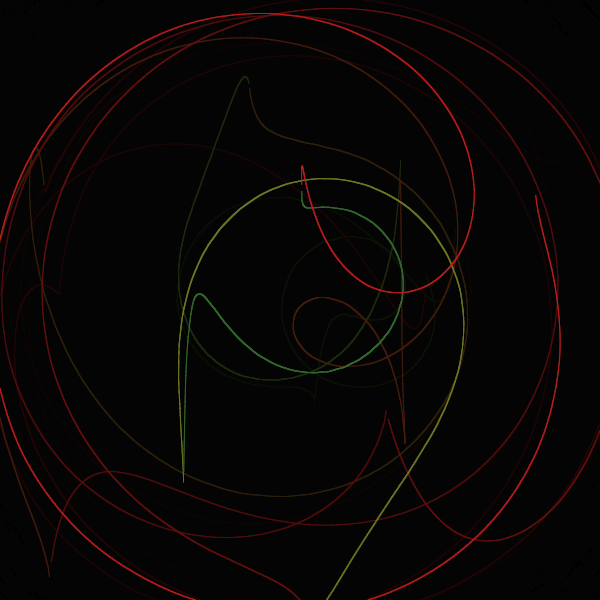
\includegraphics[width=0.44\textwidth]{images/blake2.png}
	\label{fig:blake}
}
\subfigure[Debussy -- Prelude a l'apres-midi d'un faune: Orchestral]{
	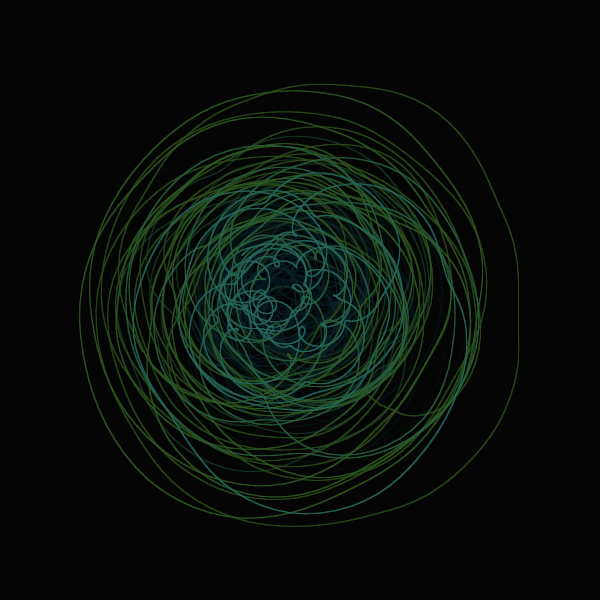
\includegraphics[width=0.44\textwidth]{images/debussy.png}
	\label{fig:debussy}
}
\subfigure[Flogging Molly -- Grace Of God Go I: Solo male voice]{
	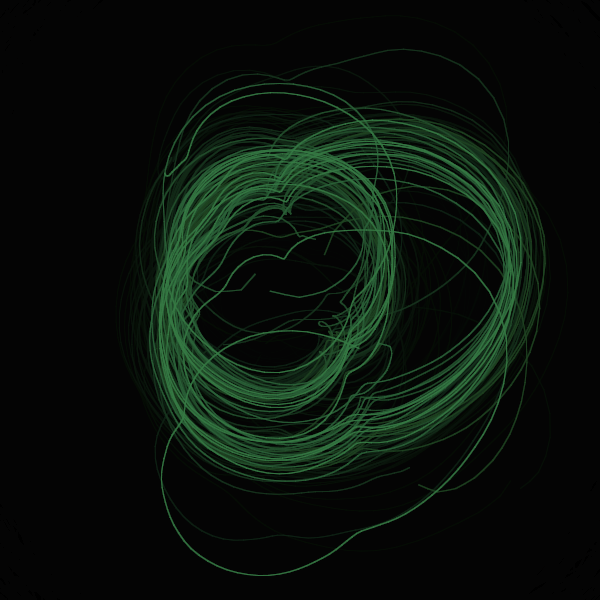
\includegraphics[width=0.44\textwidth]{images/grace.png}
	\label{fig:grace}
}
\subfigure[86Hz oscillator with partials 1--8 at various levels]{
	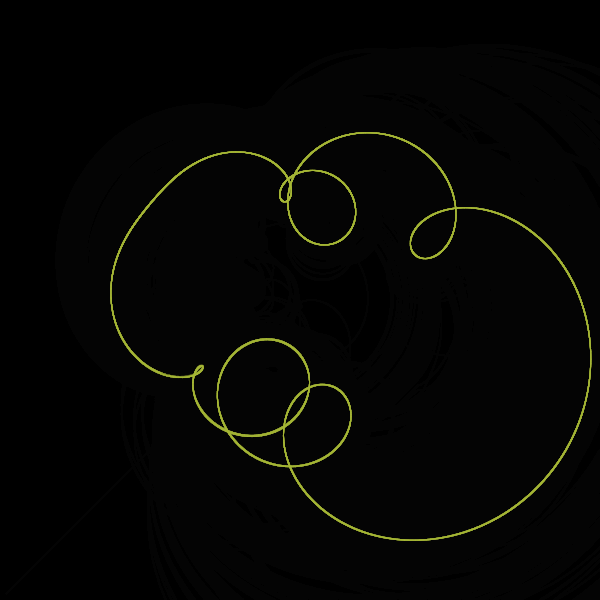
\includegraphics[width=0.44\textwidth]{images/wave.png}
	\label{fig:wave}
}
\label{fig:examples}
\caption{Screenshots taken from real--time audio streams}
\end{figure}

\newpage

\section{Full code listing}
\label{app:code}
\lstset{
  language=Python,                % the language of the code
  basicstyle=\footnotesize\ttfamily,           % the size of the fonts that are used for the code
  numbers=left,                   % where to put the line-numbers
  numberstyle=\tiny\color{gray},  % the style that is used for the line-numbers
  stepnumber=1,                   % the step between two line-numbers. If it's 1, each line will be numbered
  numbersep=5pt,                  % how far the line-numbers are from the code
  backgroundcolor=\color{white},      % choose the background color. You must add \usepackage{color}
  showspaces=false,               % show spaces adding particular underscores
  showstringspaces=false,         % underline spaces within strings
  showtabs=false,                 % show tabs within strings adding particular underscores
  frame=none,                   % adds a frame around the code
  rulecolor=\color{black},        % if not set, the frame-color may be changed on line-breaks within not-black text (e.g. commens (green here))
  tabsize=4,                      % sets default tabsize to 2 spaces
  captionpos=b,                   % sets the caption-position to bottom
  breaklines=true,                % sets automatic line breaking
  breakatwhitespace=false,        % sets if automatic breaks should only happen at whitespace
  keywordstyle=\color{blue},          % keyword style
  commentstyle=\color{dkgreen},       % comment style
  stringstyle=\color{mauve},         % string literal style
}
\lstinputlisting{../round_visualizer2.py}

\end{appendix}


\end{document}  